\documentclass[psfig,preprint]{aastex}
\begin{document}
 
%\documentclass[preprint]{aastex}
%\usepackage{graphicx}

\title{BPIDL---BASIC PLOTTING IN IDL: \\ 
PLOTS, MULTIPLE PLOTS, COLORS, MAKING POSTSCRIPT FILES \\ \today}

\author{Carl Heiles, Tim Robishaw} 

This is an introduction to plotting in IDL. We also cover some
embellishments: arrays of plots, 4d plots using symbol size and color,
selecting groups of plotted points with the cursor. And we discuss how
to make good-looking PostScript plots for papers and talks.  This
document is only an {\it introduction}: you can do almost anything on
plotting with IDL!

\tableofcontents

\section{PLOTTING BASICS}

\subsection{The {\tt plot} Command}

We can call {\tt plot} with several keywords and optional inputs.
The top panel of Figure \ref{fig1} is the plot generated by the following
commands\footnote{The \$ symbol tells IDL that the command is continuing on the
next line; we use multiple lines for clarity in this introduction.}:

\begin{verbatim}
plot, xdata, ydata, psym=7, $
xrange=[0,10], yrange=[0,22], xstyle=1, ystyle=1, $
xtitle='x-axis label (units)', $
ytitle='y-axis label (units)', $
title='Global Title'
\end{verbatim}

\begin{figure} [!ht]
\begin{center}
\includegraphics[scale=0.6]{bpfig1.ps}
%\includegraphics{bpfig1.ps}
\caption{An example plot illustrating overplotting, use of color,
  errorbars, annotating with {\tt xyouts} and also with {\tt legend},
  math and Greek with {\tt textoidl}, and making arrays of plots with
  IDL's native {\tt !p.multi} .\label{fig1}}
\end{center}
\end{figure}

Comparing the plot with the command should make it clear which options
did what. A few comments: \begin{enumerate}

\item The optional input {\tt psym=7} defined the plotting symbol; there
  are many others available\footnote{Specifically, {\tt
      [psym=[0,1,2,3,4,5,6,7,8]} are [plus, asterisk, period, diamond,
        triangle, square, X, user-defined, undefined, histogram
        mode]. An easy way to define your own symbols is with GSFC's
      {\tt plotsym}, which gives you [arrows, a star, triangle,
        upside-down triangle, square, circle]; and lets you fill them in
      if you want; for its documentation, type {\tt doc, 'plotsym'} .},
    which you can obtain from IDL's online help (type {\tt ?plot} while
    in IDL).  When {\tt psym} is set to a negative number, the points
    are plotted and, also, connected by lines.

\item {\tt (xy)range}: setting these equal to a two element vector
  causes the plot ranges to be set to the values in those vectors.  For
  {\tt x}, the (first, second) elements are the (left, right) axis
  limits and for {\tt y}, the (bottom, top). So when you are plotting
  things versus right ascension, which astronomers always plot backwards
  (high numbers on the left instead of the right), you specify this with
  the {\tt xrange} vector.

\item {\tt (xy)style}: Normally, the x and y ranges are rounded to make
  human-comfortable numbers (like 10 instead of 9.5).  Setting these
  {\tt styles} to unity forces the ranges to be exactly what you
  specify. There are lots of other options for the {\tt style} keywords.
\end{enumerate}

\subsection{Overplotting} \label{oplot}

We use the {\tt oplot} command to overlay other plots on top of ones we
have already made and display the results on the middle panel of Figure
\ref{fig1}.  Let's plot a fitted dashed line through our data; and just
for fun, we color it red:

\noindent {\tt oplot, xtheory, ytheory, linestyle=2, color=!red}

\noindent Here {\tt linestyle=2} produces a dashed line. Our startup
file predefines 12 colors ({\tt !red, !blue, etc}; look at the printout
when IDL starts up). Let's overplot some errorbars, too:

\noindent {\tt oploterr, xdata, ydata, yerrors}

\noindent There are other ways to plot error bars: {\tt errplot} and
          {\tt ploterr}. And you can plot errorbars in the x-direction
          with our {\tt errplot\_x}. Finally, the less used but highly
          functional {\tt plots} command overplots an individual point,
          or an array of points, all with different colors and/or
          symbols if you wish (e.g., \S \ref{annotating}).

\subsection{Annotating Plots} \label{annotating}

The {\tt xyouts} command lets you annotate plots. In the example below, {\tt
xyouts, 7.0, 6.5, 'data points'} writes the string {\tt data points}
beginning at the specified locations of (x,y) = (7.0, 6.5). You can
locate the annotation in data coordinates, normalized coordinates
(relative to the plot box), or device coordinates (pixels); see the
documentation. 

You can add legends to your plots using {\tt plots} and {\tt xyouts}.
The legends on lower-right in Figure \ref{fig1} were made with the
following commands:

\begin{verbatim}
plots, 6.8, 6.7, ps=7
xyouts, 7.0, 6.5, 'data points'
plots, [6.5,6.9], [5.5,5.5], lines=2
xyouts, 7.0, 5.4, 'theory'
plots, [6.8,6.8], [4.0,4.5]
xyouts, 7.0, 4.2, 'error bars'
\end{verbatim}

That's the hard way!  The easy way: use GSFC's {\tt legend} command. To
see its documentation, type {\tt doc, 'legend'} in IDL. In Figure
\ref{fig1}, for the legend on upper-left of the bottom panel:

\begin{verbatim}
items= ['data points', 'theory', 'error bars']
psym=[7,0,0]
lines=[0, 3, 0]
legend, items, lines=lines, psym=psym, position=[1.5, 16.0]
\end{verbatim}

\subsection{You Want Greek Letters or Math? Use {\tt textoidl}}

Figure \ref{fig1}, bottom panel also has some math annotation. There are
two ways to do Greek letters and sub/superscripting.  One is IDL's
native embedded formatting, which is infinitely flexible and
consequently complicated; the other is the popular non-native procedure
{\tt textoidl}, which lets you use \TeX\ notation to generate fancy IDL
character strings.  That's how we annotated Figure \ref{fig1} with the
string $Density^2 / Radius_1^3 \leq \gamma$:
\begin{verbatim}
xyouts, 4, 2, textoidl('Density^2 / Radius_1^3 \leq \gamma'
\end{verbatim}

\noindent If this looks like Greek to you, then you don't know
\TeX. As a scientist, you'll need to learn it!
 
\section{MAKING ARRAYS OF PLOTS}

\subsection{Arrays of plots using IDL's {\tt !p.multi} System Variable}\label{pmulti}

The {\tt !p.multi} system variable in IDL allows you to place multiple
plots into the same window\footnote{{\tt !p.multi} is an IDL system
  variable because it is prepended by a ! . System variables are always
  accessible, whether you are at the main level or in any procedure or
  function. Some other noteworthy system variables are {\tt !pi, !dtor,
    !radeg} . And in our startup file we define colors, such as {\tt
    !red}, as system variables. }.  To accomplish this, set {\tt
  !p.multi} equal to a three-element vector with the first element zero,
the second element equal to the number of plots across the window and
the third element equal to the number of plots down the window.  Then
give your plotting commands.  For example, our Figure \ref{fig1} was
made like this:

\begin{figure}[!ht]
\begin{center}
\includegraphics[scale=0.6]{bpfig2.ps}
\caption{The same plots as in Figure \ref{fig2}. The array was made 
with {\tt multiplot} . \label{fig2}}
\end{center}
\end{figure}

\begin{verbatim}
!p.multi=[0,1,3]
plot, xd, yd, psym=7...
;other commands for this plot...

plot, xd, yd, psym=7...
;other commands for this plot...

plot, xd, yd, psym=7...
;other commands for this plot...

!p.multi=0
\end{verbatim}

\subsection{Arrays of plots using GSFC's {\tt multiplot}} \label{multiplot}

{\tt !p.multi} allows enough space around each plot for its own axis
titles, and a plot title. Often, the x-axes and/or the y-axes have
identical titles or scales. In such cases, the space around each plot is
annoying and wasteful. You can eliminate it by using GSFC's {\tt
  multiplot.pro}; for its documentation, type {\tt doc, 'multiplot'} if
you use our startupfile or, if you don't, type {\tt doc\_library,
  'multiplot'}. Figure \ref{fig2}, which has the same content as Figure
\ref{fig1}, was made like this:

\begin{verbatim}
multiplot, /init

multiplot,[1,3]
plot, xd, yd, psym=7, xstyle=1, title=title ...
;other commands for this plot...

multiplot
plot, xd, yd, psym=7, xstyle=1 ...
;other commands for this plot...

multiplot
plot, xd, yd, psym=7, xstyle=1, xtitle=xtitle ...
multiplot,/reset
;other commands for this plot...
\end{verbatim}

\noindent Note the trick: you can't write a global title (with {\tt
  title}) except on the top plot of a column, and you can't write an {\tt
  xtitle} on any plot except the bottom---you don't want the x-axis
information in the lower plot area! For the same reason, {\tt multiplot}
automatically suppresses the numbers on the x-axis for all plots other
than the bottom one.

\section{USE DIFFERENT-STYLED POINTS TO REPRESENT A THIRD (OR
  FOURTH! OR FIFTH!) VARIABLE}

Sometimes you want to represent a third variable with the plot-point
style. For example, your data points might come from different
years. You can use different {\tt psym} values or different symbol sizes
to get differently-shaped
points. 

\begin{figure}[!ht]
\begin{center}
\includegraphics[scale=0.8]{colorpntplt.ps}
\caption{A 4-d plot (in which each point represents four different
  quantities). To make any sense at all, this plot {\it must} be viewed
  in color! \label{colorpntplt}}
\end{center}
\end{figure}

Alternatively, you can use color, and have a colorbar tell what the colors
mean. And you can even represent {\it four} variables using {\it both}
{\tt psym} and color! And you can represent {\it five} using symbol
size, shape, and color! The easy way is with our home-grown procedure
{colorpntplt.pro}. Figure \ref{colorpntplt} was made like this:

\begin{verbatim}
;FIRST, CONSTRUCT A USER-DEFINED SQUARE, FILLED-IN PLOT SYMBOL...
plotsym, 8, 1, /fill

;MAKE AN ARRAY OF SYMBOL SIZES PROPORTIONAL TO SOURCE FLUX DENSITIES...
symsize= (tx.flux < 2) + 0.4

;MAKE THE PLOT...
colorpntplt, ell, bee, tx, xra=[360, 0], yra=[-20,90.], zra=[0,100], $
xtit='Gal Long', ytit='Gal Lat', ztit='Tspin', tit='Symsize is flux', $
psym=8, symsize=symsize, /bg

;SETTING bg ABOVE FILLS THE PLOT ``background'' WITH GRAY, WHICH IS
;       OFTEN GOOD FOR COLORS.
\end{verbatim}

\noindent Two important points: \begin{enumerate}
\item What color scheme to use for the plotted points? Here, we follow
  the philosophy that all colors should be perceived as being of equal
  brightness. This results in a color scheme that uses nonsaturated
  colors. For details, see \S 3.2 in the handout ``1d2d3d: One, Two, and
  Three Dimensional Color Images''.

\item What background color for the plot? Note we use gray. This has the
  great advantage of having good contrast with all relevant
  colors---even both black and white!
\end{enumerate}

\section{SELECTING GROUPS OF POINTS IN A PLOT}

Often, after you plot some points, you wonder about a few that occupy a
region of the plot space. We have two procedures than enable you to
select groups of points. One, {\tt pointsinside.pro}, uses the cursor;
the other, {\tt graphselect.pro}, selects the points within a curve you
plot using the {\tt oplot} command. Try them!

\section{FOR DOCUMENTS AND TALKS, USE POSTSCRIPT} \label{doctalks}

IDL makes exportable images in many formats, but the one you'll use for
most purposes is PostScript. It's best because, uniquely, its images are
pixelized, but its characters are vectorized. This means that characters
are drawn using lines whose placement is limited only by the resolution
of the plotting device, not the resolution imposed by finite-sized
pixels. To do PostScript the easy way, see \S \ref{easyps} below.

\subsection{Don't Ignore the Aesthetics!}\label{psfiles}
Your documents and talks are your link to the world and it is important
to make this link as clear and attractive as possible. Think of all the
PowerPoint illegible graphs and text you've had to sit through in a dark
room with a boring speaker who rushes from one slide tto the next
without explaining what the axes are on his illegible graphs! 

There's an art---based human physiology, document printing technology,
and PowerPoint technology---to making plots and images that are easily
read and absorbed into the human psyche.  To this
end, {\it fonts, characcter size, symbol size,} and {\it line thickness}
are {\bf very important!} IDL's default font is meant for computer
screens: it's fast and legible when you're up close. Ditto for it's
default line thickness and, usually, character sizes. But they're not so
great for the finished product.

For example, compare the two plots below. Which is more
legible---especially when projected on a screen during a talk? It's easy
to do this right. We've written a crude wrapper called {\tt ps\_ch.pro}
to set quantities to values that are suitable for most purposes; it
replaaces {\tt psopen} and {\tt psclose}. Here's how it's used:
\begin{verbatim}                                                                            
ps_ch, 'psfilename.ps', /defaults, /color, xsize=8, ysize=8, /inch                          
                                                                                            
[put your plot and imaging commmands
  here]                                                  
                                                                                            
ps_ch, /close                                                                               
\end{verbatim}

\noindent You might not like it's defaults; you can change them, or
write your own following the style in this procedure.

\begin{figure}[h!]
\begin{center}
\includegraphics[scale=.6]{ps_ch0_rainbowplot.ps}
\includegraphics[scale=.6]{ps_ch1_rainbowplot.ps}
\end{center}
\caption{Plots from PostScript files. The left-hand one uses default
  fonts and thicknesses; the right-hand one uses non-default ones.
  \label{fig}}
\end{figure}

\subsection{Some cautionary words about color.} 

Unnecessary use of
color is a no-no because lots of people are colorblind---about 15\% of
males. The most common form of colorblindness is the inability to
distinguish red from green. Physiologically, a non-colorblind eye has
three types of receptors---red, green, and blue---and these seem like
the natural colors to use. However, instead of red and green, use
magenta (red + blue) and cyan (blue + green); red/green colorblind
people find these easier to distinguish. Even better: don't use color at
all! Instead, distinguish
different types of points and lines using {\tt psym} and {\tt
  linestyle}. Or, if you must use color, {\it also} use {\tt psym} and {\tt
  linestyle}!

I recommend the following websites: \begin{enumerate}

\item {\tt
  http://www.nature.com/nature/journal/v445/n7128/full/445593c.html} 
        (Comments by an annoyed colorblind proposal reviewer)

\item {\tt http://colororacle.cartography.ch/}
        (Download software to see how a colorblind person sees your stuff)

\item {\tt http://colorfilter.wickline.org/}
        (Measure the readability of your stuff)
\end{enumerate}

Generally, you need to use contrasting colors that are easily
distinguishable. The highest contrast comes with a primary color and its
complement---e.g., [white (red+green+blue) {\it vs.}\ black
  (white--(red+green+blue))]; [magenta (red+blue) {\it vs.}\ green
(white--(red+blue)); [cyan (green+blue) {\it vs.}\ red
  (white--(green+blue))]; [yellow (red+green) {\it vs.}\ blue
  (white--(red+green))].  You can get away with somewhat less contrasty
combinations.

But {\it stay away} from the {\it least} contrasting color
combinations. Remember that the eye is not very sensitive to blue
light. So blue on black is almost unreadable. Ditto for the
complementary pair, yellow on white. Too many PowerPoint slides show a
bunch of curves in different colors and the most important is
yellow. Plotted on a white background, it is almost invisible. How many
speakers have said ``Sorry that the most important curve is so hard to
see on this slide\dots''---as if they couldn't do anything about it!
When the speaker made the original plot, it was probably on the black
background of the computer screen, where yellow looks terrific!

\section{TWO EASY WAYS TO MAKE PostScript} \label{easyps}

IDL has native routines, but we recommend our wrappers\footnote{For more
  information about PostScript, see our tutorial ``PSIDL---Postscript
  Files in IDL\dots''.}. Here's what you do: 

\subsubsection{The easier way}

If you're not that much of a perfectionist and want something
adequate, easy, and quick (that's me!), then\dots

\begin{enumerate}

\item Open the PostScript device, making sure to specify the x- and
  y-sizes; this determines the aspect ratio of your PostScript window.

\noindent {\tt ps\_ch, 'xray.ps', /defaults, /color,
    xsize=8, ysize=8, /inch }

\item At this point, redefine the defaults set by {\tt ps\_ch} if you so
  desire. 

\item Display the image, using the same commands you used for your X
  window (your computer screen). 

\item Now close the PostScript device with {\tt ps\_ch, /close} . This
  also resets all of the defaults.
\end{enumerate}


\subsubsection{The slightly less easy way}

\begin{enumerate}
\item Open the PostScript device, making sure to specify the x- and
  y-sizes; this determines the aspect ratio of your PostScript window.

\noindent {\tt psopen, 'xray.ps', /times, /bold, /isolatin1, /color,
    xsize=8, ysize=8, /inch }
\noindent {\tt setcolors, /sys}

\noindent This defines the output for your plot to be the PS file {\tt
  xray.ps}, uses the Times/Bold font, allows color in the image (you
don't need {\tt /color} or the {\tt setcolors} command for a
black-and-white plot), and sets the x and y sizes to 8 and 8 inches.

\item Set character sizes, line thicknesses, and font appropriately. You
  can do this by specifying them within the plot and other commands;
  alternatively, you use our preferred method, which is to set system
  variables before plotting and then reset them afterwards. 

If you're a perfectionist, you'll use larger sizes and thicker lines for
PowerPoint than you will for a paper document. If you're lazy, you can
use our wrapper for {\tt psopen}, called {\tt ps\_ch} (see below); if
you're not lazy, you can use {\tt ps\_ch} as a model for how you set the
system variables.

\item Display the image, using the same commands you used for your X
  window (your computer screen). 

\item Now close the PostScript device and return to X windows and its
  colortable: 
\begin{verbatim}
psclose
setcolors, /sys
\end{verbatim}
\end{enumerate}

\section {QUICK AND DIRTY: WRITING SCREEN PIXELS TO
  POSTSCRIPT}
\label{dirty}

Above we described how to make elegant, beautiful PostScript
images.  It requires rerunning the plot/imaging commands.  Here we
describe the quick and dirty way, which does {\it not} require
rerunning: you first generate the X window version; then you read the
image pixels directly from the screen and turn them into a PostScript
file.  Using our procedures, this is quick and totally painless.
However, the output looks ratty for text and graphs, which consist of
lines; pixelized lines don't look very good.  But you may be willing to
put up with this sometimes---if you're in a hurry, or making a hardcopy
for your lab notebook, for example.  If you want to use this quick and
dirty technique but want better-looking results, use a larger window;
the pixelization on the hardcopy will be less noticeable.

        This consists of two subsections, one for plots and one for
images.  For plots, we assume grayscale with either two levels (1
bit---black and white) or 256 levels (8 bits---grayscale; some plots
have shading).  If your color table has fewer than 256 levels, we
interpolate it to 256; this is great for grayscale, but if you are
using a non-gray color table it will probably give you weird
results.

        Both procedures retain the aspect ratio on the window, even if
you try to change it with the keywords.  If you want a different aspect
ratio, then generate a new window with the desired aspect ratio (using
IDL's {\tt window, xsize=256, ysize=512}, for example) or rewrite the
procedure for yourself.

\subsection{Copying plots with {\tt hardplot}}

We assume you've already generated your plot, which is displayed in an
IDL window.  If necessary, select this window using IDL's {\tt wset}
command.  Then type

\noindent {\tt hardplot}

\noindent It will ask for the name of the output filename.  {\tt 
hardplot} is a home-grown procedure that has keywords that allow you to
do various things.  The default values are set for reproducing ordinary
black/white plots, {\it inverting the white-on-black that you see on
your screen to the black-on-white that you should use for a printed
output.} 

\subsection{Copying images with {\tt hardimage}}

{\tt hardimage} reproduces the X window display faithfully to the
PostScript file.  It's almost identical to {\tt hardplot} running with
{\tt nbits=8} and the {\tt noreverse} option, but it also copies the
colors if the image is not grayscale.


\end{document}
